\documentclass[12pt]{article}
\usepackage{cite}
\usepackage[a4paper, margin=1in]{geometry}
\usepackage{graphicx}
\usepackage[utf8]{inputenc}
\usepackage{subcaption}
\usepackage{placeins}
\usepackage{wrapfig}
\usepackage{float}
\usepackage{hyperref}
\usepackage{minted}
\usepackage{amsmath}
\usepackage{mathtools}
\usepackage{algorithm}
\usepackage[noEnd=false, indLines=false]{algpseudocodex}
\usepackage{setspace}
\usepackage{times}
\usepackage{tikzit}
% \documentclass[12pt]{article}
\usepackage{cite}
\usepackage[a4paper]{geometry}
\usepackage{graphicx}
\usepackage[utf8]{inputenc}
\usepackage{subcaption}
\usepackage{placeins}
\usepackage{wrapfig}
\usepackage{float}
\usepackage{hyperref}
\usepackage{minted}
\usepackage{amsmath}
\usepackage{mathtools}
\usepackage{algorithm}
\usepackage[noEnd=false, indLines=false]{algpseudocodex}
\usepackage{setspace}
\usepackage{times}
\usepackage{tikzit}
% \documentclass[12pt]{article}
\usepackage{cite}
\usepackage[a4paper]{geometry}
\usepackage{graphicx}
\usepackage[utf8]{inputenc}
\usepackage{subcaption}
\usepackage{placeins}
\usepackage{wrapfig}
\usepackage{float}
\usepackage{hyperref}
\usepackage{minted}
\usepackage{amsmath}
\usepackage{mathtools}
\usepackage{algorithm}
\usepackage[noEnd=false, indLines=false]{algpseudocodex}
\usepackage{setspace}
\usepackage{times}
\usepackage{tikzit}
% \documentclass[12pt]{article}
\usepackage{cite}
\usepackage[a4paper]{geometry}
\usepackage{graphicx}
\usepackage[utf8]{inputenc}
\usepackage{subcaption}
\usepackage{placeins}
\usepackage{wrapfig}
\usepackage{float}
\usepackage{hyperref}
\usepackage{minted}
\usepackage{amsmath}
\usepackage{mathtools}
\usepackage{algorithm}
\usepackage[noEnd=false, indLines=false]{algpseudocodex}
\usepackage{setspace}
\usepackage{times}
\usepackage{tikzit}
% \input{report.tikzstyles}

\graphicspath{{./images/}}

\title{Q-learning}
\author{
  Mițca Dumitru\\
  Grupa 1406A
}
\date{2025}

\begin{document}
\maketitle

\hypersetup{linkbordercolor=1 1 1}
\tableofcontents
\hypersetup{linkbordercolor=1 0 0}

\singlespacing
\newpage

\section{Proposed problem}

This year of University I have entered the NXP Cup Competition, in which me and my team must
create an autonomous car with the goal of finishing an unknown track in as little time
as possible without leaving the bounds of the tracks, which are signaled by black lines.

In this paper, I will explore the possible application of Q-Learning in this domain.

\begin{figure}
  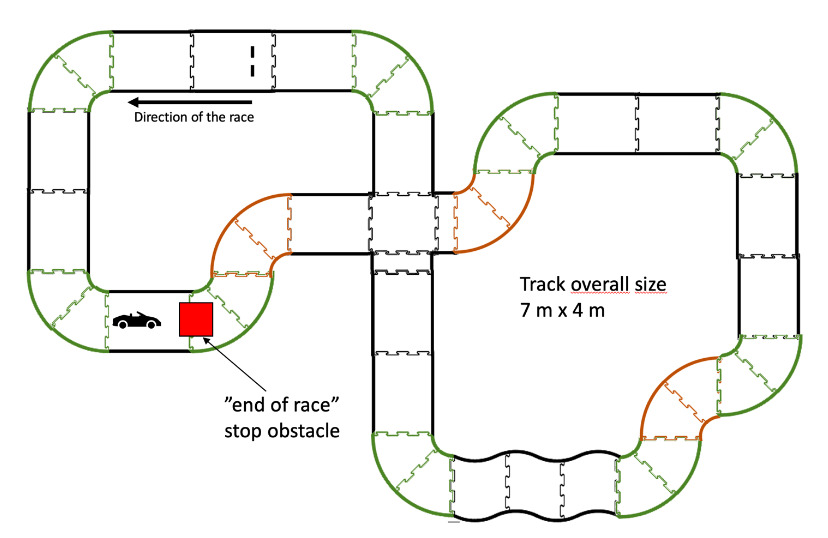
\includegraphics[width=\linewidth]{nxp-track}
  \caption{An example track\protect\footnotemark}
\end{figure}

\footnotetext{The "end of race" stop obstacle is added after the car has completed two laps} \cite[p.~9]{NxpCupRules:2025}

\newpage

\section{Algorithm}

Q-learning is a widely used reinforcement learning approach, used in domains such as game theory,
network communications, and robotics\cite{8836506}.

The goal of the agent is to maximise the total rewards it receives from the environment\cite{reinforcementlearningintro}.
\begin{align*}
  G_T = \sum_{\mathclap{k=0}}^{\infty} \gamma^{k} R_{t+k+1}
\end{align*}

We introduce a state-value function  which estimates how good being at a state $s$ is under a policy $\pi$:
\begin{align*}
  v(s) = E_{\pi}\left[\sum_{\mathclap{k=0}}^{\infty}\gamma^{k} R_{t+k+1} \mid S_t = s\right]
\end{align*}

We can then introduce an action-value function which estimates how good taking an action $a$ during a state $s$ is under a policy $\pi$:
\begin{align*}
  q(s, a) = E_{\pi}\left[\sum_{\mathclap{k=0}}^{\infty}\gamma^{k} R_{t+k+1} \mid S_t = s, A_t = a\right]
\end{align*}

We can now introduce the following Bellman equation, which our agent must maximise:
\begin{align*}
  Q(S_t, a_t) \gets (1 - \alpha) \underbrace{Q(S_t, a_t)}_{\text{current value}} + \alpha * \underbrace{(\underbrace{R_{t+1}}_{reward} + \gamma \max_{a'}{Q(S_{t+1}, a')})}_{\text{new value}}
\end{align*}

We propose the following algorithm, based on \cite[p.~67--72]{AICourse13} and \cite{qlearningalgo}:

\begin{algorithm}[H]
  \caption{Q-Learning algorithm}
  \textbf{Data:}
  \begin{itemize}
    \item $E$ --- The environment in which the agent resides
  \end{itemize}
  \textbf{Algorithm parameters:}
  \begin{itemize}
    \item $\alpha$ --- the learning rate
    \item $\gamma$ --- discount factor
    \item $\epsilon$ --- probability of exploring the environment
    \item $N_e$ --- number of episodes
    \item $N_i$ --- number of iterations per episode
  \end{itemize}
  \begin{algorithmic}
    \Procedure{QLearning}{$E$}
    \Require $\alpha, \epsilon \in \left[0, 1 \right]$, $\gamma \in \left(0, 1\right]$

    \State Initialize $Q(S, a)$, where $Q$ is a data table holding the possible reward for state $S$ and action $a$

    \For{$e \gets 0$ \textbf{to} $N_e$}
    \State $S \gets$ \Call{Reset}{$E$}

    \For{$i \gets 0$ \textbf{to} $N_i$}
    \State $a \gets$ \Call{PickAction}{$E$, $S$, $\epsilon$}
    \If{\Call{IsTerminal}{$a$}}
    \State Exit inner loop
    \EndIf
    \State take action $a$, observe reward $R$ and next state $S'$
    \State $Q(S, a) \gets (1 - \alpha)Q(S, a) + \alpha * (R + \gamma \max_{a'}{Q(S', a')})$
    \State $S \gets S'$
    \EndFor

    \EndFor

    \EndProcedure
  \end{algorithmic}
\end{algorithm}

\section{Proposed solution}
We propose to solve the problem by implementing the above algorithm in python, and creating
a text-based format for representing the map.
\section{Source code listings}

\section{Results}

\newpage

\bibliography{refs}
\bibliographystyle{ieeetr}

\section*{Individual contributions}
This project was realised solely by me, and I attest the code I have written is my own.

\end{document}


\graphicspath{{./images/}}

\title{Q-learning}
\author{
  Mițca Dumitru\\
  Grupa 1406A
}
\date{2025}

\begin{document}
\maketitle

\hypersetup{linkbordercolor=1 1 1}
\tableofcontents
\hypersetup{linkbordercolor=1 0 0}

\singlespacing
\newpage

\section{Proposed problem}

This year of University I have entered the NXP Cup Competition, in which me and my team must
create an autonomous car with the goal of finishing an unknown track in as little time
as possible without leaving the bounds of the tracks, which are signaled by black lines.

In this paper, I will explore the possible application of Q-Learning in this domain.

\begin{figure}
  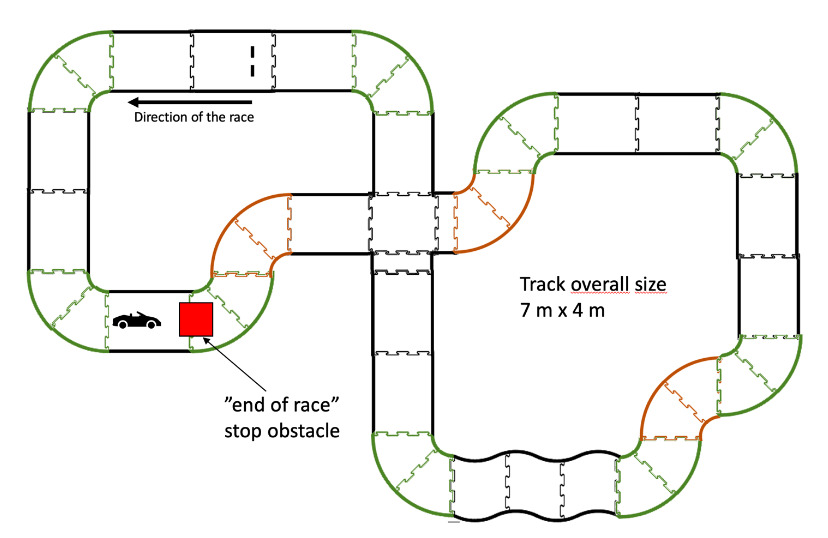
\includegraphics[width=\linewidth]{nxp-track}
  \caption{An example track\protect\footnotemark}
\end{figure}

\footnotetext{The "end of race" stop obstacle is added after the car has completed two laps} \cite[p.~9]{NxpCupRules:2025}

\newpage

\section{Algorithm}

Q-learning is a widely used reinforcement learning approach, used in domains such as game theory,
network communications, and robotics\cite{8836506}.

The goal of the agent is to maximise the total rewards it receives from the environment\cite{reinforcementlearningintro}.
\begin{align*}
  G_T = \sum_{\mathclap{k=0}}^{\infty} \gamma^{k} R_{t+k+1}
\end{align*}

We introduce a state-value function  which estimates how good being at a state $s$ is under a policy $\pi$:
\begin{align*}
  v(s) = E_{\pi}\left[\sum_{\mathclap{k=0}}^{\infty}\gamma^{k} R_{t+k+1} \mid S_t = s\right]
\end{align*}

We can then introduce an action-value function which estimates how good taking an action $a$ during a state $s$ is under a policy $\pi$:
\begin{align*}
  q(s, a) = E_{\pi}\left[\sum_{\mathclap{k=0}}^{\infty}\gamma^{k} R_{t+k+1} \mid S_t = s, A_t = a\right]
\end{align*}

We can now introduce the following Bellman equation, which our agent must maximise:
\begin{align*}
  Q(S_t, a_t) \gets (1 - \alpha) \underbrace{Q(S_t, a_t)}_{\text{current value}} + \alpha * \underbrace{(\underbrace{R_{t+1}}_{reward} + \gamma \max_{a'}{Q(S_{t+1}, a')})}_{\text{new value}}
\end{align*}

We propose the following algorithm, based on \cite[p.~67--72]{AICourse13} and \cite{qlearningalgo}:

\begin{algorithm}[H]
  \caption{Q-Learning algorithm}
  \textbf{Data:}
  \begin{itemize}
    \item $E$ --- The environment in which the agent resides
  \end{itemize}
  \textbf{Algorithm parameters:}
  \begin{itemize}
    \item $\alpha$ --- the learning rate
    \item $\gamma$ --- discount factor
    \item $\epsilon$ --- probability of exploring the environment
    \item $N_e$ --- number of episodes
    \item $N_i$ --- number of iterations per episode
  \end{itemize}
  \begin{algorithmic}
    \Procedure{QLearning}{$E$}
    \Require $\alpha, \epsilon \in \left[0, 1 \right]$, $\gamma \in \left(0, 1\right]$

    \State Initialize $Q(S, a)$, where $Q$ is a data table holding the possible reward for state $S$ and action $a$

    \For{$e \gets 0$ \textbf{to} $N_e$}
    \State $S \gets$ \Call{Reset}{$E$}

    \For{$i \gets 0$ \textbf{to} $N_i$}
    \State $a \gets$ \Call{PickAction}{$E$, $S$, $\epsilon$}
    \If{\Call{IsTerminal}{$a$}}
    \State Exit inner loop
    \EndIf
    \State take action $a$, observe reward $R$ and next state $S'$
    \State $Q(S, a) \gets (1 - \alpha)Q(S, a) + \alpha * (R + \gamma \max_{a'}{Q(S', a')})$
    \State $S \gets S'$
    \EndFor

    \EndFor

    \EndProcedure
  \end{algorithmic}
\end{algorithm}

\section{Proposed solution}
We propose to solve the problem by implementing the above algorithm in python, and creating
a text-based format for representing the map.
\section{Source code listings}

\section{Results}

\newpage

\bibliography{refs}
\bibliographystyle{ieeetr}

\section*{Individual contributions}
This project was realised solely by me, and I attest the code I have written is my own.

\end{document}


\graphicspath{{./images/}}

\title{Q-learning}
\author{
  Mițca Dumitru\\
  Grupa 1406A
}
\date{2025}

\begin{document}
\maketitle

\hypersetup{linkbordercolor=1 1 1}
\tableofcontents
\hypersetup{linkbordercolor=1 0 0}

\singlespacing
\newpage

\section{Proposed problem}

This year of University I have entered the NXP Cup Competition, in which me and my team must
create an autonomous car with the goal of finishing an unknown track in as little time
as possible without leaving the bounds of the tracks, which are signaled by black lines.

In this paper, I will explore the possible application of Q-Learning in this domain.

\begin{figure}
  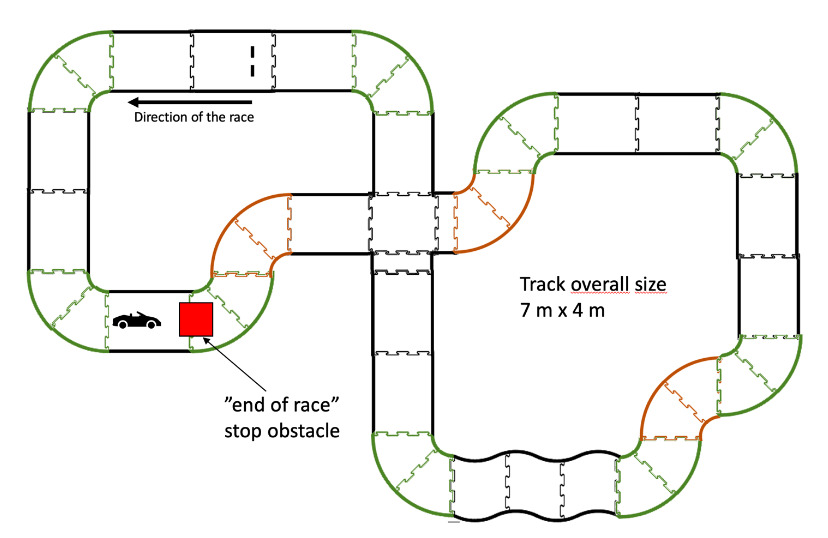
\includegraphics[width=\linewidth]{nxp-track}
  \caption{An example track\protect\footnotemark}
\end{figure}

\footnotetext{The "end of race" stop obstacle is added after the car has completed two laps} \cite[p.~9]{NxpCupRules:2025}

\newpage

\section{Algorithm}

Q-learning is a widely used reinforcement learning approach, used in domains such as game theory,
network communications, and robotics\cite{8836506}.

The goal of the agent is to maximise the total rewards it receives from the environment\cite{reinforcementlearningintro}.
\begin{align*}
  G_T = \sum_{\mathclap{k=0}}^{\infty} \gamma^{k} R_{t+k+1}
\end{align*}

We introduce a state-value function  which estimates how good being at a state $s$ is under a policy $\pi$:
\begin{align*}
  v(s) = E_{\pi}\left[\sum_{\mathclap{k=0}}^{\infty}\gamma^{k} R_{t+k+1} \mid S_t = s\right]
\end{align*}

We can then introduce an action-value function which estimates how good taking an action $a$ during a state $s$ is under a policy $\pi$:
\begin{align*}
  q(s, a) = E_{\pi}\left[\sum_{\mathclap{k=0}}^{\infty}\gamma^{k} R_{t+k+1} \mid S_t = s, A_t = a\right]
\end{align*}

We can now introduce the following Bellman equation, which our agent must maximise:
\begin{align*}
  Q(S_t, a_t) \gets (1 - \alpha) \underbrace{Q(S_t, a_t)}_{\text{current value}} + \alpha * \underbrace{(\underbrace{R_{t+1}}_{reward} + \gamma \max_{a'}{Q(S_{t+1}, a')})}_{\text{new value}}
\end{align*}

We propose the following algorithm, based on \cite[p.~67--72]{AICourse13} and \cite{qlearningalgo}:

\begin{algorithm}[H]
  \caption{Q-Learning algorithm}
  \textbf{Data:}
  \begin{itemize}
    \item $E$ --- The environment in which the agent resides
  \end{itemize}
  \textbf{Algorithm parameters:}
  \begin{itemize}
    \item $\alpha$ --- the learning rate
    \item $\gamma$ --- discount factor
    \item $\epsilon$ --- probability of exploring the environment
    \item $N_e$ --- number of episodes
    \item $N_i$ --- number of iterations per episode
  \end{itemize}
  \begin{algorithmic}
    \Procedure{QLearning}{$E$}
    \Require $\alpha, \epsilon \in \left[0, 1 \right]$, $\gamma \in \left(0, 1\right]$

    \State Initialize $Q(S, a)$, where $Q$ is a data table holding the possible reward for state $S$ and action $a$

    \For{$e \gets 0$ \textbf{to} $N_e$}
    \State $S \gets$ \Call{Reset}{$E$}

    \For{$i \gets 0$ \textbf{to} $N_i$}
    \State $a \gets$ \Call{PickAction}{$E$, $S$, $\epsilon$}
    \If{\Call{IsTerminal}{$a$}}
    \State Exit inner loop
    \EndIf
    \State take action $a$, observe reward $R$ and next state $S'$
    \State $Q(S, a) \gets (1 - \alpha)Q(S, a) + \alpha * (R + \gamma \max_{a'}{Q(S', a')})$
    \State $S \gets S'$
    \EndFor

    \EndFor

    \EndProcedure
  \end{algorithmic}
\end{algorithm}

\section{Proposed solution}
We propose to solve the problem by implementing the above algorithm in python, and creating
a text-based format for representing the map.
\section{Source code listings}

\section{Results}

\newpage

\bibliography{refs}
\bibliographystyle{ieeetr}

\section*{Individual contributions}
This project was realised solely by me, and I attest the code I have written is my own.

\end{document}


\graphicspath{{./images/}}

\title{Q-learning}
\author{
  Mițca Dumitru\\
  Grupa 1406A
}
\date{2025}

\begin{document}
\maketitle

\hypersetup{linkbordercolor=1 1 1}
\tableofcontents
\hypersetup{linkbordercolor=1 0 0}

\singlespacing
\newpage

\section{Proposed problem}

This year of University I have entered the NXP Cup Competition, in which me and my team must
create an autonomous car with the goal of finishing an unknown track in as little time
as possible without leaving the bounds of the tracks, which are signaled by black lines.

In this paper, I will explore the possible application of Q-Learning in this domain.

\begin{figure}[H]
  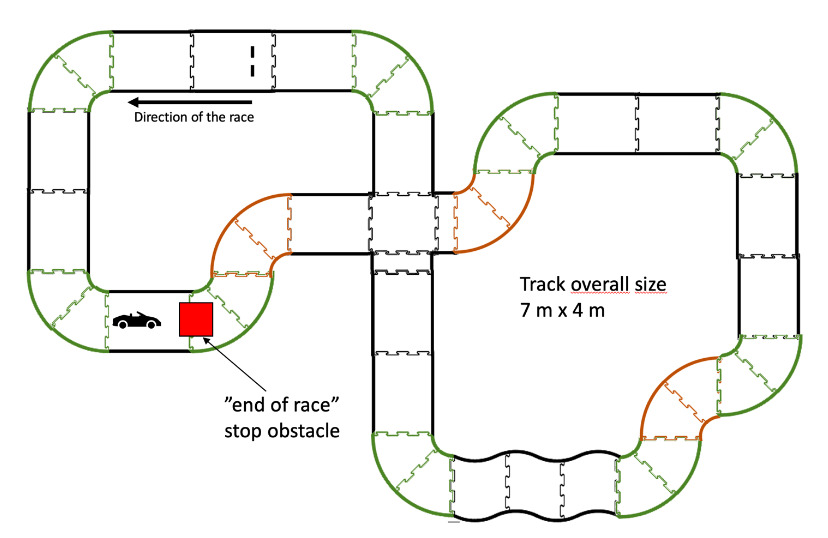
\includegraphics[width=\linewidth]{nxp-track}
  \caption{An example track\protect\footnotemark}
\end{figure}

\footnotetext{The "end of race" stop obstacle is added after the car has completed two laps \cite[p.~9]{NxpCupRules:2025}}

\newpage

\section{Algorithm}

Q-learning is a widely used reinforcement learning approach, used in domains such as game theory,
network communications, and robotics\cite{8836506}.

The goal of the agent is to maximise the total rewards it receives from the environment\cite{reinforcementlearningintro}.
\begin{align}
  G_T = \sum_{\mathclap{k=0}}^{\infty} \gamma^{k} R_{t+k+1}
\end{align}

We introduce a state-value function  which estimates how good being at a state $s$ is under a policy $\pi$:
\begin{align}
  v(s) = E_{\pi}\left[\sum_{\mathclap{k=0}}^{\infty}\gamma^{k} R_{t+k+1} \mid S_t = s\right]
\end{align}

We can then introduce an action-value function which estimates how good taking an action $a$ during a state $s$ is under a policy $\pi$:
\begin{align}
  q(s, a) = E_{\pi}\left[\sum_{\mathclap{k=0}}^{\infty}\gamma^{k} R_{t+k+1} \mid S_t = s, A_t = a\right]
\end{align}

We can now introduce the following Bellman equation, which our agent must maximise:
\begin{align}\label{eqopt}
  Q(S_t, a_t) \gets (1 - \alpha) \underbrace{Q(S_t, a_t)}_{\text{current value}} + \alpha * \underbrace{(\underbrace{R_{t+1}}_{reward} + \gamma \max_{a'}{Q(S_{t+1}, a')})}_{\text{new value}}
\end{align}

We propose the following algorithm, based on \cite[p.~67--72]{AICourse13} and \cite{qlearningalgo}:

\begin{algorithm}[H]
  \caption{Q-Learning algorithm}
  \textbf{Data:}
  \begin{itemize}
    \item $E$ --- The environment in which the agent resides
  \end{itemize}
  \textbf{Algorithm parameters:}
  \begin{itemize}
    \item $\alpha$ --- the learning rate
    \item $\gamma$ --- discount factor
    \item $\epsilon$ --- probability of exploring the environment
    \item $N_e$ --- number of episodes
    \item $N_i$ --- number of iterations per episode
  \end{itemize}
  \begin{algorithmic}
    \Procedure{QLearning}{$E$}
    \Require $\alpha, \epsilon \in \left[0, 1 \right]$, $\gamma \in \left(0, 1\right]$

    \State Initialize $Q(S, a)$, where $Q$ is a data table holding the possible reward for state $S$ and action $a$

    \For{$e \gets 0$ \textbf{to} $N_e$}
    \State $S \gets$ \Call{Reset}{$E$}

    \For{$i \gets 0$ \textbf{to} $N_i$}
    \State $a \gets$ \Call{PickAction}{$E$, $S$, $\epsilon$}
    \If{\Call{IsTerminal}{$a$}}
    \State Exit inner loop
    \EndIf
    \State take action $a$, observe reward $R$ and next state $S'$
    \State $Q(S, a) \gets (1 - \alpha)Q(S, a) + \alpha * (R + \gamma \max_{a'}{Q(S', a')})$
    \State $S \gets S'$
    \EndFor

    \EndFor

    \EndProcedure
  \end{algorithmic}
\end{algorithm}

\section{Proposed solution}
We propose to solve the problem by implementing the above algorithm in python, and creating
a text-based format for representing the map. Additionally we provide our agent with its
starting position\footnote{Represented as a red square in the graphical view} and the goal position\footnote{Represented
as a yellow square in the graphical view}

\begin{figure}[H]

  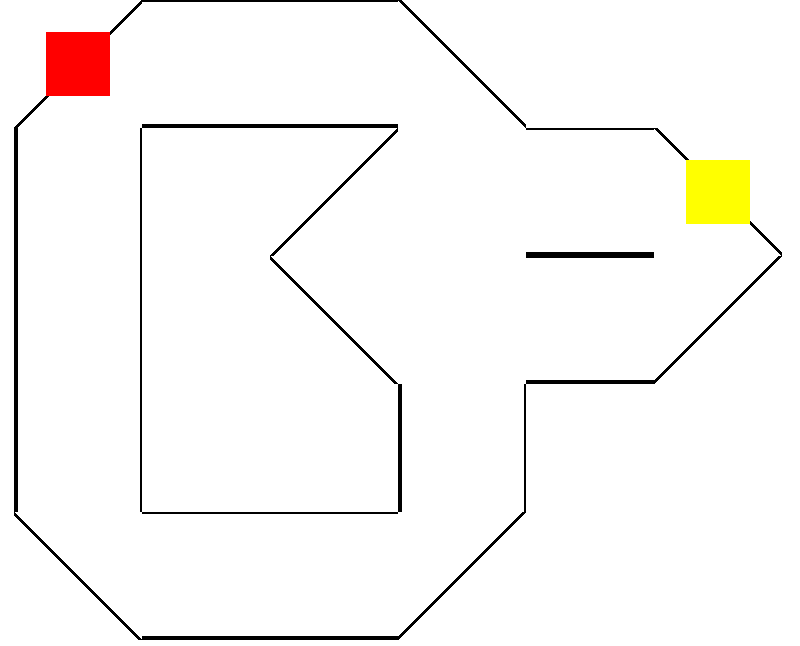
\includegraphics[width=\linewidth]{map}
  \caption{An example map used for testing the algorithm}
\end{figure}

The textual representation is the following (the newlines are part of the format)
\begin{center}
  \texttt{03224000\\0103+240\\0106+250\\01001000\\06225000}

\end{center}

\section{Source code listings}

The code of the application is structured in a manner inspired by OpenAI's Gym
\footnote{"A toolkit for developing and comparing reinforcement learning algorithms." \url{https://github.com/openai/gym}} Python library\cite{1606.01540}

\subsection{Environment object}
The Python program contains a \texttt{QLEnvironment} class which provides the following interface for
the agent to interact with the environment:

\begin{minted}[breaklines]{python3}
class QLEnvironment:
  def reset(self) -> float:
    ...

  def _position_to_state(self, x: float, y: float) -> float:
    ...

  @property
  def n_actions(self) -> float:
    ...

  @property
  def n_observations(self) -> float:
    ...

  def sample_action(self) -> float:
    ...

  def step(self, action, visual: bool = False) -> tuple[float, float, bool]:
    ...

\end{minted}

The implementation detail have been ommitted as this abstraction would allow us to use different representations
for the map data itself.

\subsection{Algorithm implementation}

The algorithm is split across three functions to allow reuse of its steps between training the agent and
the visual display

\subsubsection{The iteration step}

This function optimises the equation \ref{eqopt} and implements the innermost loop of the presented algorithm.

\inputminted[firstline=78,lastline=94,autogobble,breaklines]{python}{algo.py}

\subsubsection{The episode loop}

This function implements a full iteration, it implements the rest of the presented algorithm, and lowers the
exploration probability using a negative exponential function.

It also tracks some statistics for obtaining more data about an episode.

\inputminted[firstline=45,lastline=60,autogobble,breaklines]{python}{algo.py}

\subsubsection{The training}
The agent's is trained in the following function:
\inputminted[firstline=39,lastline=43,autogobble,breaklines,breakanywhere]{python}{algo.py}

The function also records statistics to gather information for

\section{Results}

After 10000 episodes, the agent can correctly arrive at its goal.

\begin{figure}[H]
  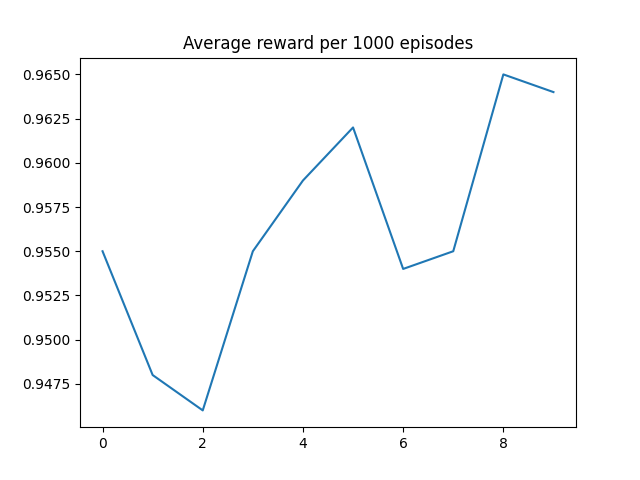
\includegraphics[width=\linewidth]{results}
  \caption{It can be observed that reward has an upwards trend with more episodes\protect\footnotemark}
  \centering
\end{figure}

\footnotetext{Graph generate using Matplotlib \cite{Hunter:2007}}

However, after implementing and researching Q-Learning, I have come to the conclusion that it is not appropriate
for the original goal of being used in an aotonoumous car in the NXP Cup competition. Q-learning looks to be more
appropriate for situations where failure is not fatal, while in the competition, leaving the track leads to losing
that attempt.

\newpage

\bibliography{refs}
\bibliographystyle{ieeetr}

\end{document}
